%summary for IMA

\documentclass[french]{article}
\usepackage[utf8]{inputenc}
\usepackage[T1]{fontenc}
\usepackage{babel}
\usepackage{lmodern}
\usepackage{graphicx}
\usepackage{tikz}
\usetikzlibrary{arrows}

\usepackage{amsmath}
\usepackage{amsfonts}

\usepackage{float}

\title{Ima}
\date{}
\author{L3 RI}


\begin{document}
\maketitle
\tableofcontents
\newpage

\section{Introduction}
On considère des images en niveaux de gris. À chaque pixel d'une image
on associe donc une valeur dans ${0\dots255}$
\subsection{Histogramme}
L'histogramme d'une image donne des informations que la densité de
chaque valeur.
\paragraph{Définition} L'histogramme d'une image $I$ est une fonction
discrète qui associe à chaque valeur d’intensité le nombre de pixels
prenant cette valeur.
$$
\begin{array}{rccl}
h_t : & {0\dots255} & \to & \mathbb{N} \\
 & n & \mapsto & \text{Card}\left\{(x,y) | I(x,y) = n\right\}\\
\end{array}
$$
\subparagraph{Remarque} Si on a une image de taille $p\times q$ alors
$\sum_{n = 0}^{255} = p*q$

\subparagraph{Propriété} L'histogramme d'une image et de sa translation
sont les mêmes. Ce n'est donc \emph{pas une caractéristique de l'image}.

\paragraph{Interprétation} Si l'histogramme est condensé sur les valeurs
faibles (resp. sur les fortes) alors l'image est \emph{sous-exposé} (resp.
\emph{surexposé}).

\paragraph{Égalisation} On peut normaliser un histogramme condensé en
étalant ces valeurs sur toute la plage $[|0, 255|]$. Cela améliore le
contraste.

Si l'image occupe déjà toute la plage on utilise un autre algorithme basé
sur l'histograme cumulé:
$$
\begin{array}{rccl}
h_c : & {0\dots255} & \to & \mathbb{N} \\
 & n & \mapsto & \text{Card}\left\{(x,y) | I(x,y) < n\right\}\\
\end{array}
$$

On répartit pour obtenir un histogramme linéaire.

\begin{figure}[h]
\begin{center}
{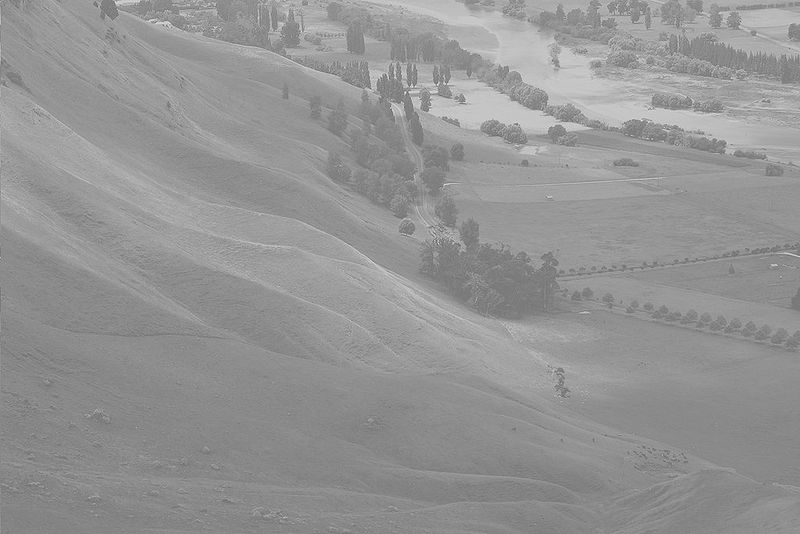
\includegraphics[scale=0.16]{images/histo01.jpg}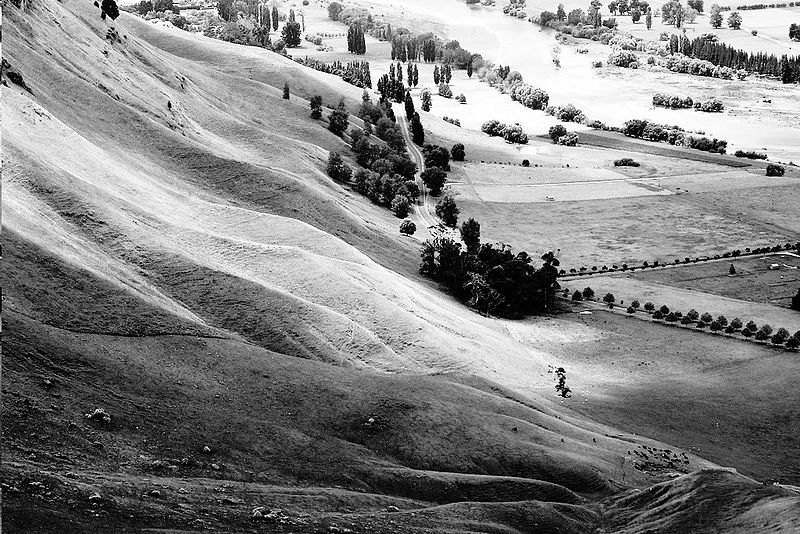
\includegraphics[scale=0.16]{images/histo03.jpg}} 
\end{center}
\begin{center}
{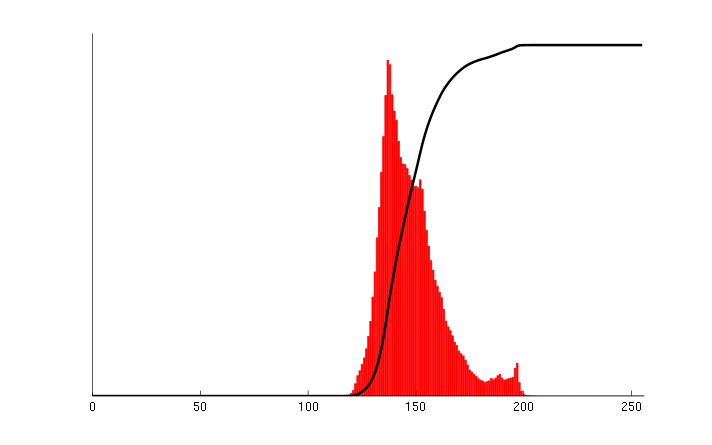
\includegraphics[scale=0.16]{images/histo02.png}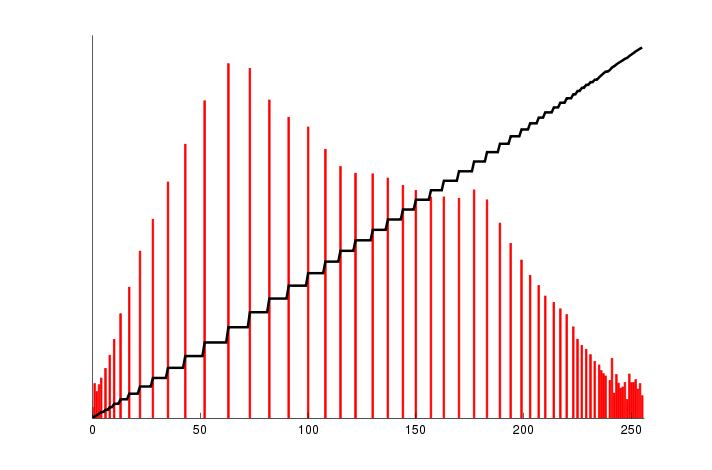
\includegraphics[scale=0.16]{images/histo04.png}} 
\end{center}
\caption{Résultat de l'Algorithme d'égalisation de l'histogramme}
(Source : Wikipédia)
\end{figure}

\subsection{Transformations géométriques}
Le résultat d'une transformation géométrique (rotation, transformations
affines, etc.) aboutit généralement à ce que les pixels de l'image
d'origine n'aient plus des coordonnées entières.

\paragraph{Inteprolation d'intensité} L'interpolation permet de déduire
la couleur des positions entières à partir des positions non entières
connues.

Exemple : Plus proches voisins, bilinéaire, bicubique, par convolution.

\paragraph{Convolution 1D}
$$(f * g)(x) = \int_{-\infty}^{+\infty}f(x-t) g(t) dt$$

\paragraph{Convolution 2D}
Soit $g$ une fonction telle que $\int_{\Bbb{R}^2}g(x,y)dxdy=1$.
On définit l'image traitée par convolution:
$$I_{\text{convol}} = I(x,y) * g(x, y) = \int_{\Omega}g(x - a, y -b) I(a,b) da db$$

L'influence des voisins sur le résultat en une position donnée va donc
dépendre du noyau de convolution $g$ utilisé. Cela permet de lisser mais
peut aussi induire du flou.

Ex : Noyau moyenneur, gaussienne, floude bougé, etc.

\subparagraph{Remarque} Pour débruiter, un filtre médian est plus
efficace qu'un filtre moyenneur.

\section{Dérivées, opérateurs, discrétisation}
Principe: Voir une image non plus comme un tableau mais comme une fonction
$f(x,y) \in [0, 255]$


\subsection{Opérateurs usuels}

\paragraph{Dérivées partielles}
On peut considérer les dérivées partielles de l'image :
$\vert \frac{\partial f}{\partial x} \vert$ et $\vert \frac{\partial f}{\partial y} \vert$

\subparagraph{Interprétation} Une dérivée partielle grande indique une forte
variation selon la direction considérée $\longrightarrow$ permet de
détecter des contours mais dans une seule direction.

\paragraph{Gradient} Le gradient de $f$ est un champ de vecteurs:
$$\vec{\text{grad}} = \nabla f =
\left(\frac{\partial f}{\partial x}, \frac{\partial f}{\partial y} \right)$$

\subparagraph{Interprétation} Le gradient en une position donne la direction
est l'intensité de la plus forte variation autour de la position. Le
vecteur est dirigé vers les valeurs fortes. On peut donc aussi détecter
les contours, en considérant sa norme.

\paragraph{Laplacien} Le laplacien de $f$ est un champ de scalaire:
$$\Delta f = \frac{\partial^2 f}{\partial x^2} + \frac{\partial^2 f}{\partial y^2}$$

\paragraph{Divergence} La divergence d'un ensemble de vecteurs
$w = (w_1, \dots w_n)$ donne une information scalaire sur la variation
du volume autour du point.
$$\text{div} w = \frac{\partial w_1}{\partial x_1} + \dots + \frac{\partial w_n}{\partial x_n} = \nabla \cdot w$$

\paragraph{Rotationnel} [À compléter, éventuellement,
pour ceux qui ont du temps, et du courage, ou une quelconque autre motivation]

\subsection{Équation aux dérivées partielles}
\paragraph{Définition} Une équation aux dérivées partielles (EDP) est un
système d'équations faisant intervenir les dérivées partielles de fonctions
qui sont les inconnues.

\paragraph{Équation de la chaleur} EDP décrivant l'évolution de la
température $T(x,y,t)$ en l'absence de contraintes extérieures.
$$\forall (x,y) \in \Omega \frac{\partial T(x,y,t)}{\partial t} = \Delta T(x,y,t)
\quad\text{et}\quad T(x,y,0) = T_0$$

Attention le laplacien ne concerne que l'espace, ie les coordonnées $x$ et $y$

En image, la température initiale $T_0$ est donnée par $f(x,y)$.

\subparagraph{Diffusion isotrope} Diffusion sans orientation préférentielle.

La diffusion induite par l'équation de la chaleur appliquée à une image
est isotrope. Au bout d'un certain temps, l'image devient flou puis s'unifie
(homogénéisation de la température).

\paragraph{Résolution 1D} La solution de l'équation de la chaleur en 1D
$$ \frac{\partial u(x,t)}{\partial t} = \frac{\partial^2 u(x,t)}{\partial x ^2}
\quad\text{avec}\quad u(x,0) = u_0(x)$$
est $$u(x,t) = G_{\sqrt{2t}}(x,t) * u_0(x)$$
où $G_{a}$ est une gausienne d'écart type $a$.

\paragraph{Résolution 2D} De même, la solution de l'équation de la
chaleur en 2D
$$ \frac{\partial u(x,y,t)}{\partial t} = \Delta u(x,y,t)
\quad\text{avec}\quad u(x,y,0) = u_0(x,y)$$
est $$u(x,y,t) = G_(x,t,\sigma (t)) * u_0(x,y)$$
où $G_(x,t,\sigma (t))$ est une gausienne d'écart type $\sigma$
proportionnel à $t$.

\paragraph{Application à une image}La diffusion est isotrope, elle floute
donc toute l'image, sans s'arrêter aux contours. On utilise donc la divergence
pour obtenir une diffusion non-linéaire \emph{anisotrope} d'une image $I$.
$$\frac{\partial I}{\partial t} = \text{div} \left(f(x,y)\nabla I \right)$$
\begin{itemize}
\item $f$ petit $\to$ divergence faible $\to$ peu de variation au cours
du temps.
\item $f$ grand $\to$ divergence grande $\to$ diffusion importante
\end{itemize}
Ainsi les zones unies sont homogénéisées mais les contours sont conservés.

\paragraph{Autre diffusion non linéaire}Perona-Malik, diffuse selon la
norme du gradient.

\subsection{Discrétisation}
Les dérivées partielles ne sont utilisables qu'en continu.

En continu, en trouve une solution analytique.
En discret, on construit une solution, étape après étape.

\paragraph{Différences finies} On peut remplacer les dérivées partielles
par des différences finies. Pour une image décrite par une grille de pixel,
on a $I(i,j) = u(i\Delta x, j\Delta y)$ où $I$ est discrète et $u$ continue,
$\Delta x$ et $\Delta y$ sont des pas de discrétisation.
La dérivée partielle peut alors être décrite par différentes formules
$$\frac{I(j + 1,j) - I(i,j)}{\Delta x} \quad \text{(Schéma arrière)}$$
ou
$$\frac{I(j - 1,j) - I(i,j)}{-\Delta x} \quad \text{(Schéma avant)} $$
ou
$$\frac{I(j + 1,j) - I(i - 1,j)}{2\Delta x} \quad \text{(Schéma centré)} $$

\subparagraph{Remarque} Généralement pour les images, on prend
$\Delta x = \Delta y = 1$.

\subparagraph{Conditions aux bords} Ce système pose la question des
conditions aux bords. Une solution est de copier en miroir les bords pour
prolonger l'image.

\subparagraph{Sensibilité au bruit} Ce type de différenciation est très
sensible au bruit. On peut augmenter la robustesse en filtrant avant de
différencier (filtre linéaire, moyenneur ou gaussien par exemple).

\paragraph{EDP} Avec cette différenciation discrète, on peut re-résoudre
l'EDP d'une variable 1D discrète
$\frac{\partial v}{\partial t} = \alpha \frac{\partial^2 v}{\partial x ^2}$.
On trouve l'approximation $u$ de $v$, pour un pas $\Delta t$
$$u_k^{n+1} = (1 - 2r)u_k^n + r(u_{k+1}^n + u_{k-1}^n)
\quad\text{avec}\quad r = \alpha \frac{\Delta t}{\Delta x^2}$$
et où $u_k^n = u(k\Delta x, n\Delta t)$ est la variable à l'étape $n$,
translatée de $k$ pas sur $x$.

\subsection{Stabilité d'un schéma numérique}
\paragraph{Analyse} Comment choisir $\Delta x$ et $\Delta t$ ? Le choix
lors de la discrétisation va reposer sur la notion de \emph{consistance}
et de \emph{stabilité}.

\paragraph{Schéma convergent} Il y a convergence si, quand $\Delta x \to 0$
et $\Delta t \to 0$, $(k\Delta x, n\Delta t) \to (x,t)\ \Rightarrow\ u_k^n \to v(t,x)$

\paragraph{Schéma consistant} Un schéma convergent est consistant si,
lorsque les pas tendent vers $0$, l'erreur de discrétisation tend vers $0$ ie
les approximations discrètes des dérivées tendent vers les dérivées continues.

\paragraph{Stabilité}Un processus de calcul séquentiel est stable si les
erreurs d'arrondis ne s'amplifient pas lors de la progression des calculs.
$$\|u^{n+1} \| \le K\|u^0\|$$

\subparagraph{Exemple} En considérant la norme $\|u^n\| = \sup_k{|u_k^n|}$,
notre schéma précédent est stable pour $r \le \frac{1}{2}$

\subparagraph{Méthode générale}La méthode de Fourier permet de prouver
la stabilité d'un processus.

\paragraph{Explicite/Implicite} Un schéma est explicite si on peut écrire
$u_k^{n+1}$ en fonction de $u_i^n$ pour un certain $i$. Il est implicite
sinon.

\section{Restauration d'images}
\subsection{Régularisation}
\subsection{Minimisation de fonctionnelle}
\subsection{Débruitage}
\subsection{Défloutage}
\subsection{Inpainting}

\section{Segmentation}
\subsection{Seuillage d'histogramme}
\subsection{Algo K-means}
\subsection{Limites algos globaux}
\subsection{Region growing}
\subsection{Split and merge}
\subsection{Méthode markovienne}
\subsection{Graph-Cuts}
\subsection{Détecteur de Canny}
\subsection{Segmentation par contours actifs}

\section{Transformée de Fourier}
\subsection{Transformée 1D}
\subsection{Transformée 2D et 2D discrète}
\subsection{Transformée sur des images}

\end{document} 

